\begin{figure}[H]
    \centering
    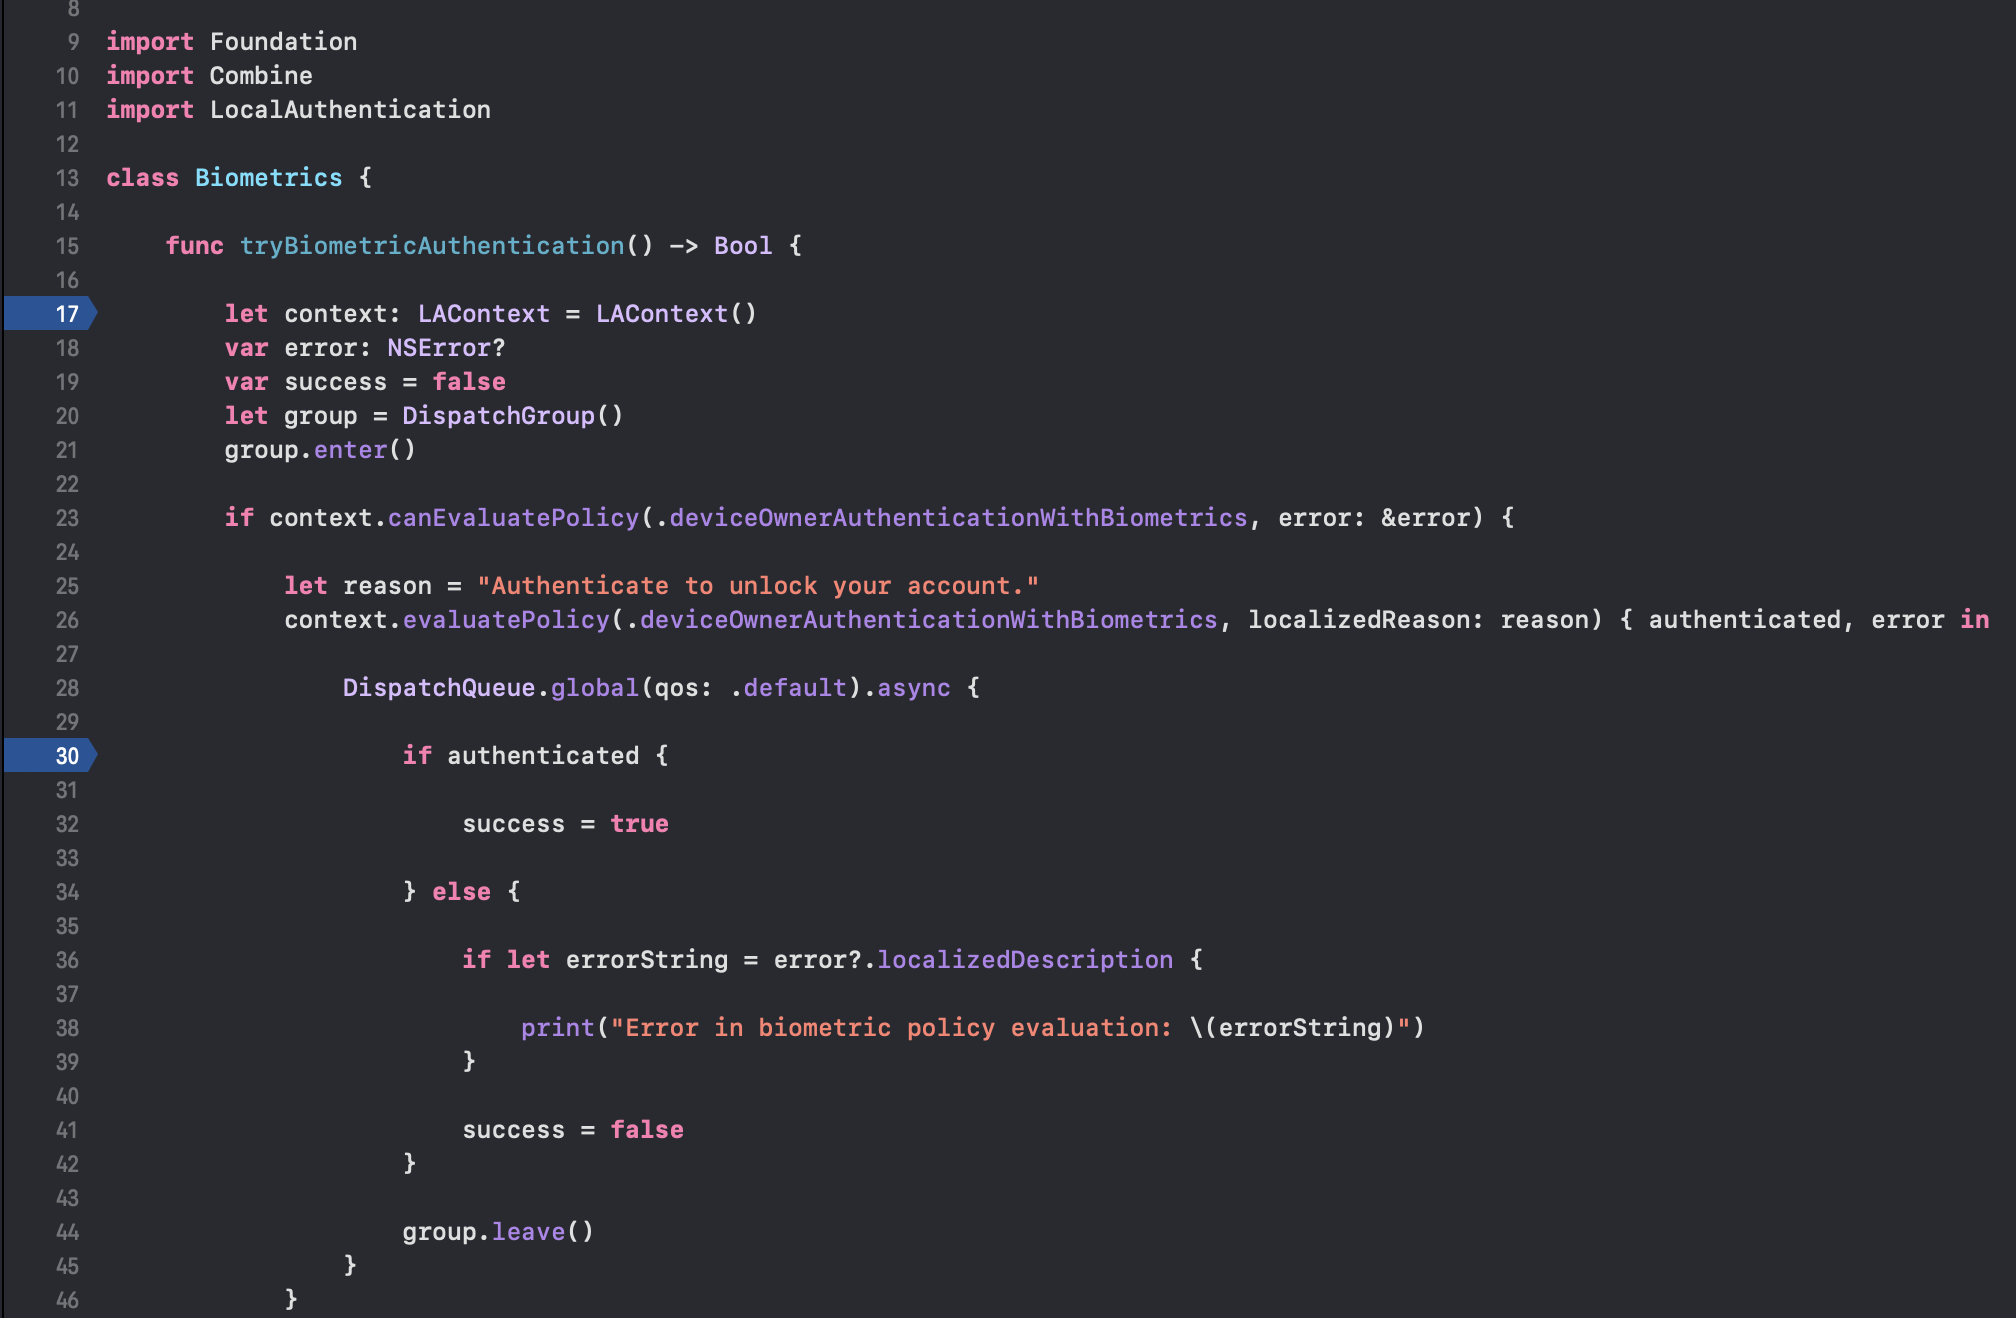
\includegraphics[width=\textwidth]{./graphics/Implementation/Settings/biometrics1.png}
    \caption{tryBiometricAuthentication() function in the Biometrics class.}
    \label{fig:biometrics1}
\end{figure}

\begin{figure}[H]
    \centering
    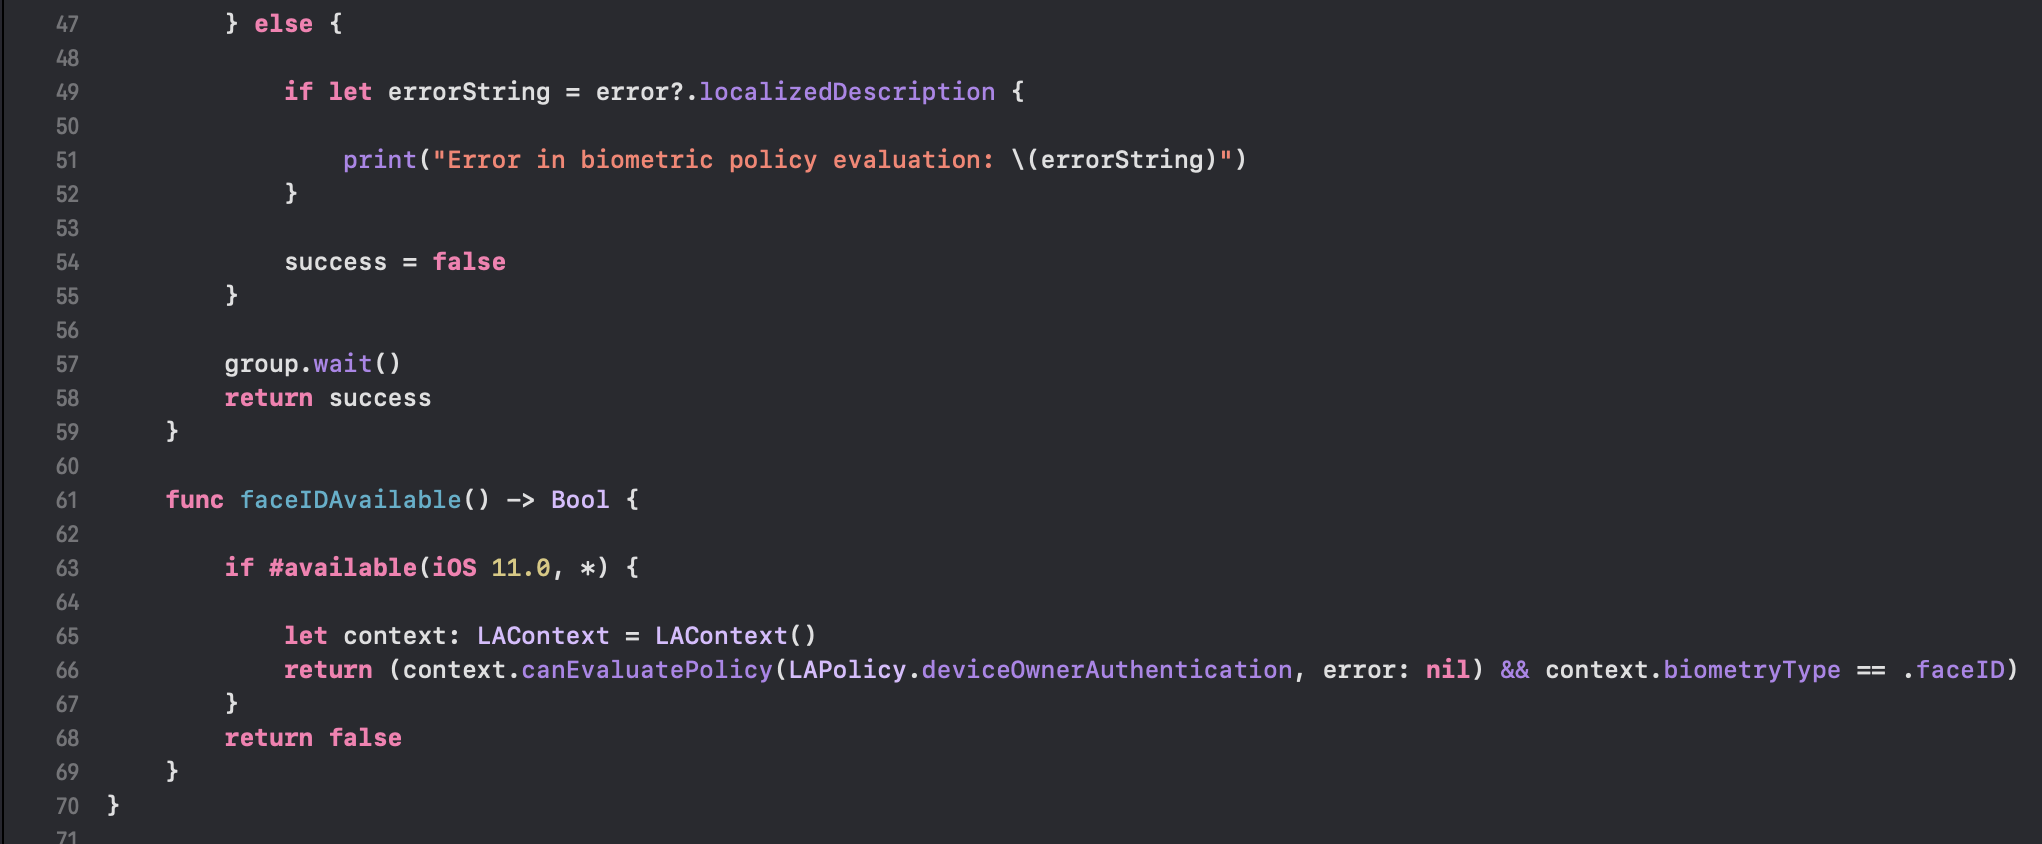
\includegraphics[width=\textwidth]{./graphics/Implementation/Settings/biometrics2.png}
    \caption{faceIDAvailable() function in the Biometrics class.}
    \label{fig:biometrics2}
\end{figure}

\begin{figure}[H]
    \centering
    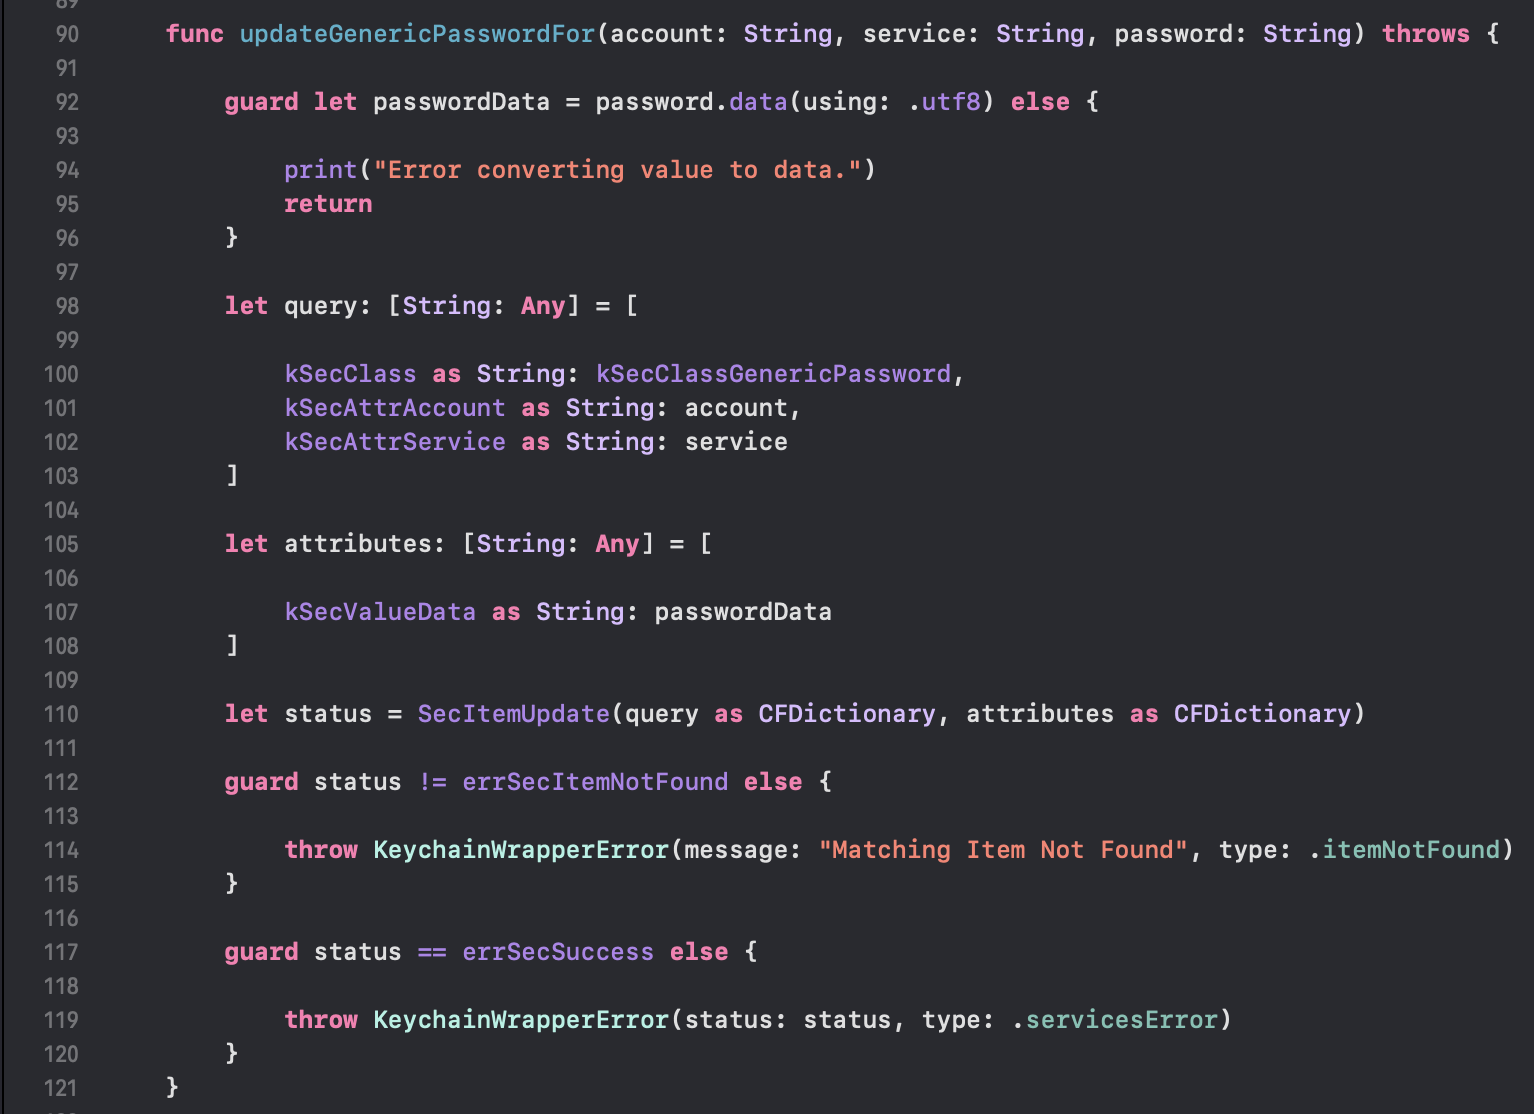
\includegraphics[width=\textwidth]{./graphics/Implementation/Settings/keychain3.png}
    \caption{updateGenericPasswordFor() function in the KeychainWrapper class.}
    \label{fig:keychain3}
\end{figure}

\begin{figure}[H]
    \centering
    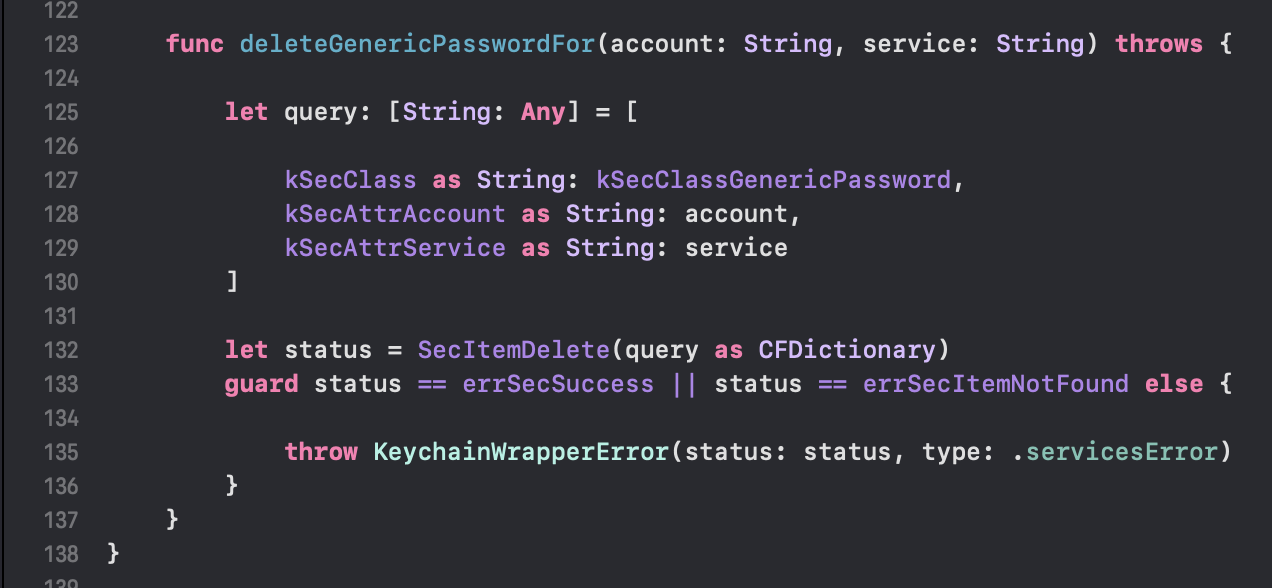
\includegraphics[width=\textwidth]{./graphics/Implementation/Settings/keychain4.png}
    \caption{deleteGenericPasswordFor() function in the KeychainWrapper class.}
    \label{fig:keychain4}
\end{figure}

\begin{figure}[H]
    \centering
    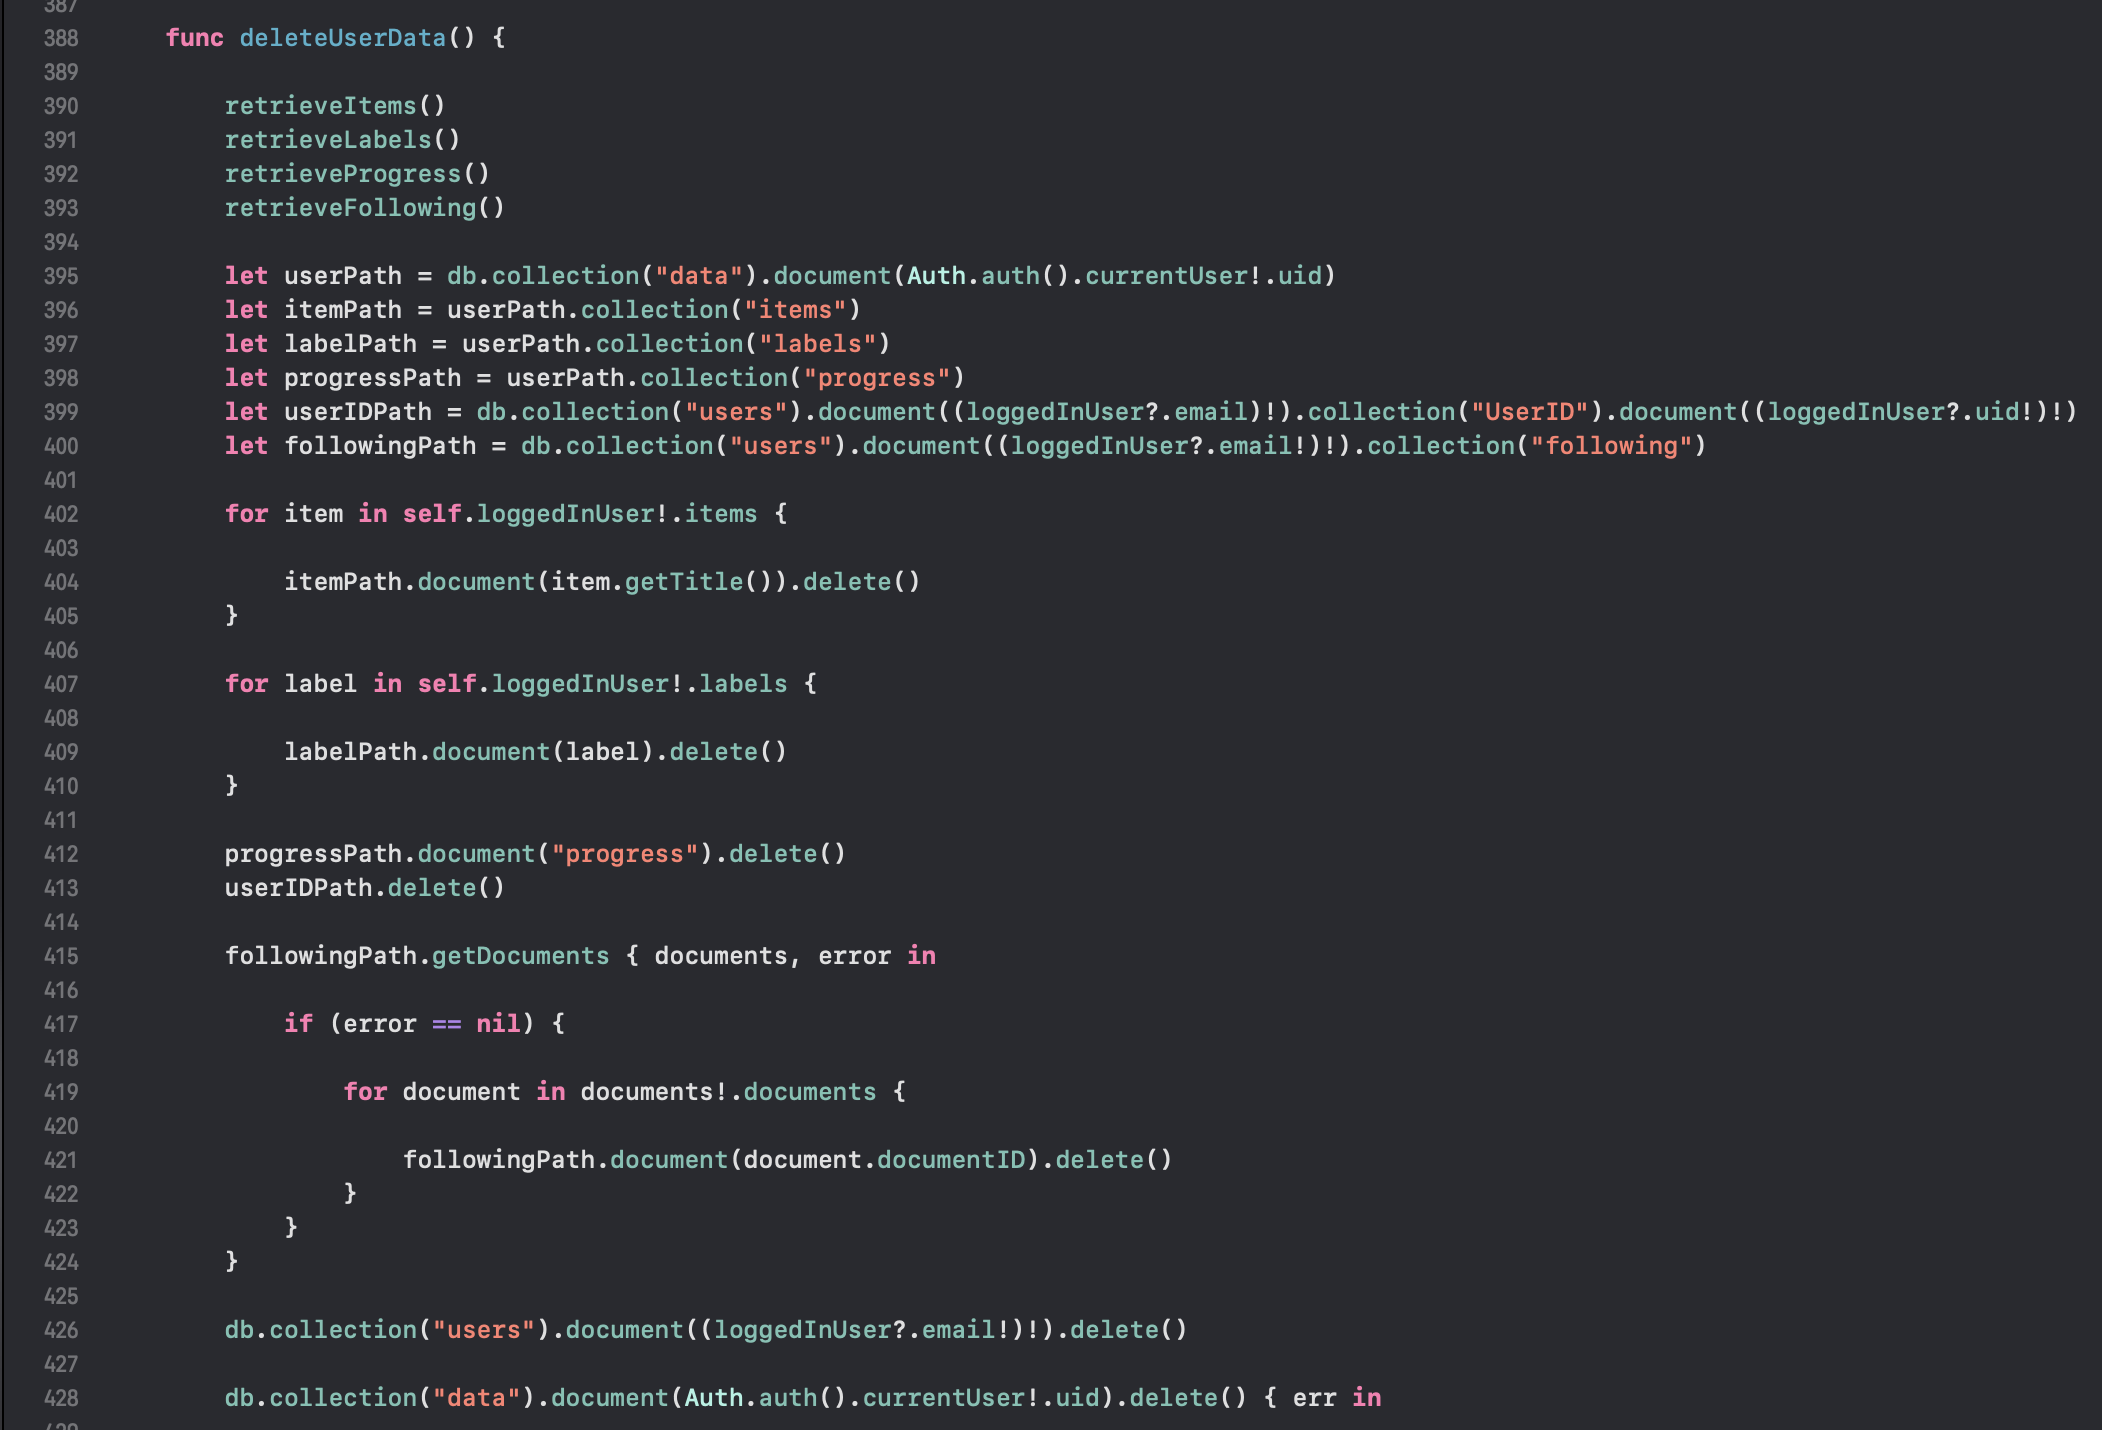
\includegraphics[width=\textwidth]{./graphics/Implementation/Settings/firebasesession1.png}
    \caption{deleteUserData() function in the FirebaseSession class.}
    \label{fig:firebasesession1_settings}
\end{figure}

\begin{figure}[H]
    \centering
    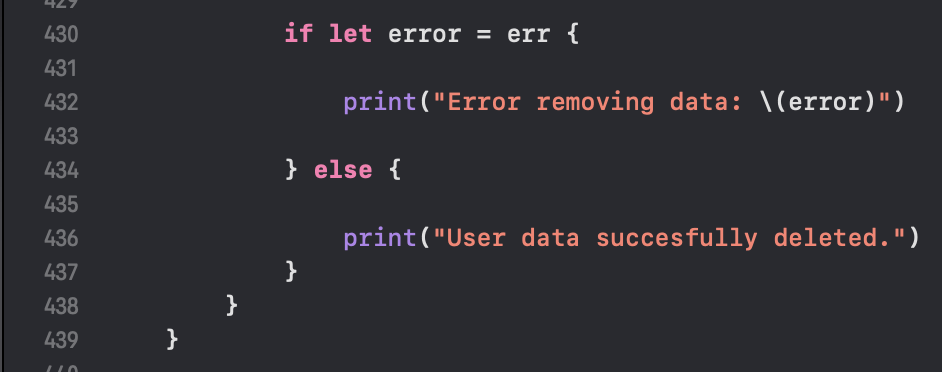
\includegraphics[width=\textwidth]{./graphics/Implementation/Settings/firebasesession2.png}
    \caption{ending of deleteUserData() function in the FirebaseSession class.}
    \label{fig:firebasesession2_settings}
\end{figure}

\begin{figure}[H]
    \centering
    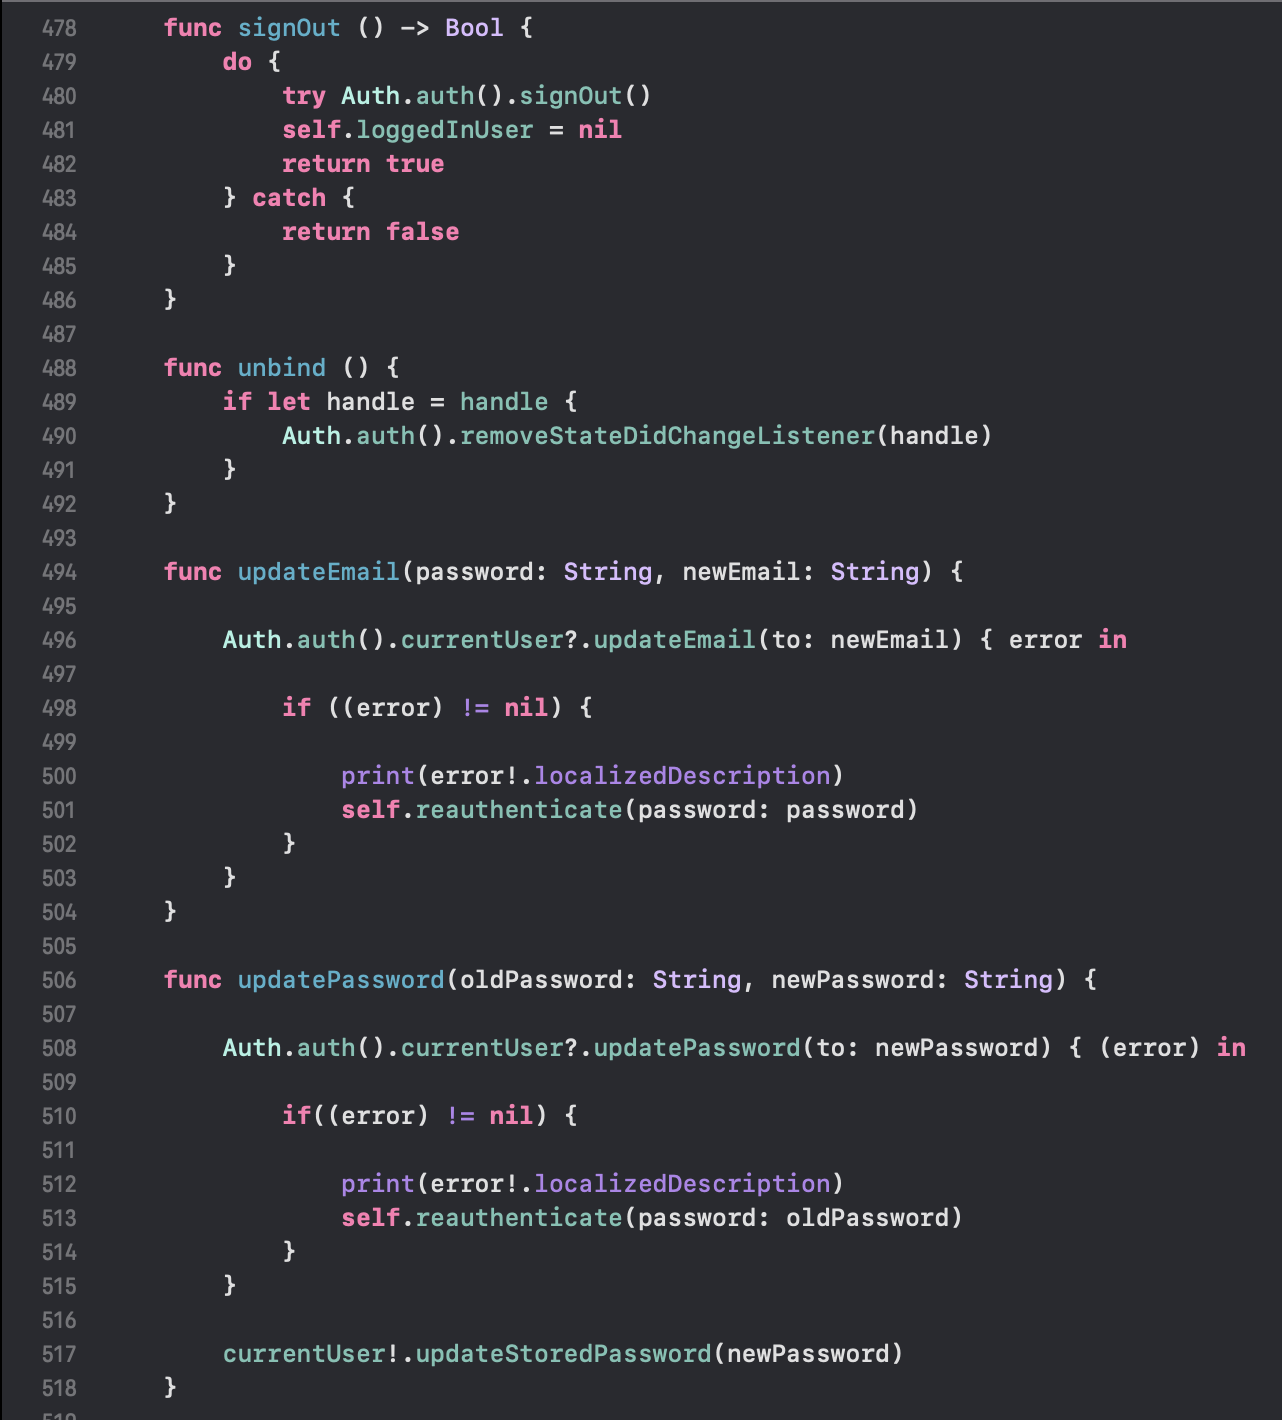
\includegraphics[width=\textwidth]{./graphics/Implementation/Settings/firebasesession3.png}
    \caption{signOut(), unbind(), updateEmail() and updatePassword() functions in the FirebaseSession class.}
    \label{fig:firebasesession3_settings}
\end{figure}

\begin{figure}[H]
    \centering
    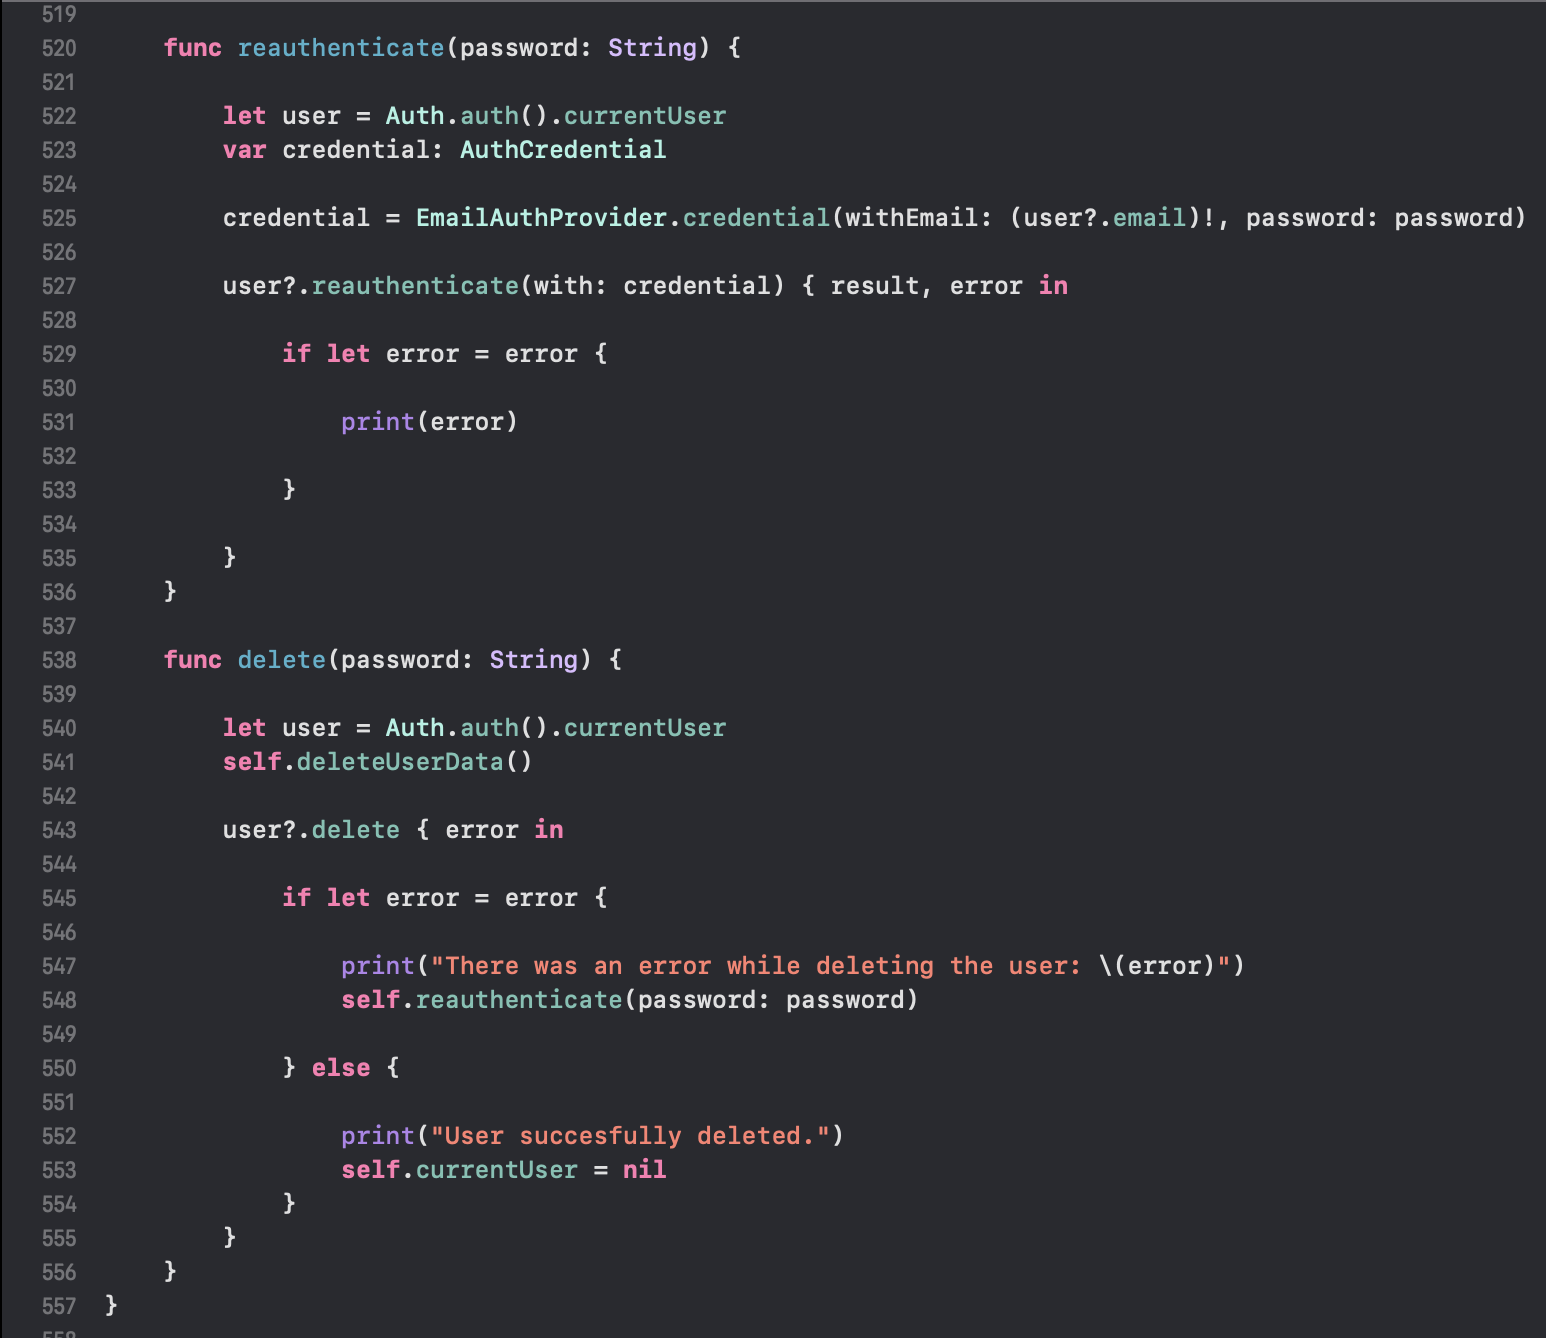
\includegraphics[width=\textwidth]{./graphics/Implementation/Settings/firebasesession4.png}
    \caption{reauthenticate() and delete() functiona in the FirebaseSession class.}
    \label{fig:firebasesession4_settings}
\end{figure}